%%%%%%%%%%%%%%%%%%%%%%%%%%%%%%%%%%%%%%%%%
% Beamer Presentation
% LaTeX Template
% Version 1.0 (10/11/12)
%
% This template has been downloaded from:
% http://www.LaTeXTemplates.com
%
% License:
% CC BY-NC-SA 3.0 (http://creativecommons.org/licenses/by-nc-sa/3.0/)
%
%%%%%%%%%%%%%%%%%%%%%%%%%%%%%%%%%%%%%%%%%

%----------------------------------------------------------------------------------------
%	PACKAGES AND THEMES
%----------------------------------------------------------------------------------------

\documentclass{beamer}

\mode<presentation> {

% The Beamer class comes with a number of default slide themes
% which change the colors and layouts of slides. Below this is a list
% of all the themes, uncomment each in turn to see what they look like.

%\usetheme{default}
%\usetheme{AnnArbor}
%\usetheme{Antibes}
%\usetheme{Bergen}
%\usetheme{Berkeley}
%\usetheme{Berlin}
%\usetheme{Boadilla}
%\usetheme{CambridgeUS}
%\usetheme{Copenhagen}
%\usetheme{Darmstadt}
%\usetheme{Dresden}
%\usetheme{Frankfurt}
%\usetheme{Goettingen}
%\usetheme{Hannover}
%\usetheme{Ilmenau}
%\usetheme{JuanLesPins}
%\usetheme{Luebeck}
\usetheme{Madrid}
%\usetheme{Malmoe}
%\usetheme{Marburg}
%\usetheme{Montpellier}
%\usetheme{PaloAlto}
%\usetheme{Pittsburgh}
%\usetheme{Rochester}
%\usetheme{Singapore}
%\usetheme{Szeged}
%\usetheme{Warsaw}

% As well as themes, the Beamer class has a number of color themes
% for any slide theme. Uncomment each of these in turn to see how it
% changes the colors of your current slide theme.

%\usecolortheme{albatross}
%\usecolortheme{beaver}
%\usecolortheme{beetle}
%\usecolortheme{crane}
%\usecolortheme{dolphin}
%\usecolortheme{dove}
%\usecolortheme{fly}
%\usecolortheme{lily}
%\usecolortheme{orchid}
%\usecolortheme{rose}
%\usecolortheme{seagull}
%\usecolortheme{seahorse}
%\usecolortheme{whale}
%\usecolortheme{wolverine}

%\setbeamertemplate{footline} % To remove the footer line in all slides uncomment this line
%\setbeamertemplate{footline}[page number] % To replace the footer line in all slides with a simple slide count uncomment this line

%\setbeamertemplate{navigation symbols}{} % To remove the navigation symbols from the bottom of all slides uncomment this line
}

\usepackage{graphicx} % Allows including images
\usepackage{booktabs} % Allows the use of \toprule, \midrule and \bottomrule in tables
\usepackage{algorithm, algorithmic}
\usepackage{boxhandler}
\usepackage{pdfpcnotes}
\usepackage{color}
\floatname{algorithm}{Algorithm}
\renewcommand{\algorithmicrequire}{\textbf{Input:}}
\renewcommand{\algorithmicensure}{\textbf{Output:}}
\newcommand{\argmax}{\mathop{\rm arg~max}\limits}
\newcommand{\argmin}{\mathop{\rm arg~min}\limits}

%----------------------------------------------------------------------------------------
%	TITLE PAGE
%----------------------------------------------------------------------------------------

\title[Optimal Bayesian Kalman Filtering with Prior Update]{Optimal Bayesian Kalman Filtering with Prior Update} % The short title appears at the bottom of every slide, the full title is only on the title page

\author{Toshinori Kitamura} % Your name
\institute[UCD] % Your institution as it will appear on the bottom of every slide, may be shorthand to save space
{
University of California Davis\\ % Your institution for the title page
\medskip
\textit{tkitamura@ucdavis.edu} % Your email address
}
\date{\today} % Date, can be changed to a custom date

\begin{document}

\begin{frame}
    \pnote{
    * 名前とタイトルを言う
    * There are lots of math in this slides, but I don't explain everything. 
    please review it if you are interested in
    }
\titlepage % Print the title page as the first slide
\end{frame}

\begin{frame}
    \pnote{
        * このプレゼンはこの目次に従って進める \\ 
        \\
        * First, I talk about the overview of this Paper \\
        * Second, I'll talk the overview of Kalman Filter \\
        * Then, go to the IBR Kalman Filter, the base of the OBKF, and Finally go to the OBKF
    }
\frametitle{Overview} % Table of contents slide, comment this block out to remove it
\tableofcontents % Throughout your presentation, if you choose to use \section{} and \subsection{} commands, these will automatically be printed on this slide as an overview of your presentation
\end{frame}

\section{What's this paper?}
\begin{frame}
    \tableofcontents[currentsection]
\end{frame}

\begin{frame}{What's this Paper?}
\begin{itemize}
    \item Introduce a new Kalman Filter: Optimal Bayesian Kalman Filter(OBKF)\cite{Dehghannasiri2018}
    \item OBKF is an advanced Kalman Filter of IBR Kalman Filter\cite{Dehghannasiri2017}
    \item OBKF exploits the measured data to estimate the true unknown value
\end{itemize}
\end{frame}
\section{Overview Kalman Filter} 
\begin{frame}
    \tableofcontents[currentsection]
\end{frame}

\subsection{Basic Idea}
\begin{frame}{Kalman Filter: Basic idea}
\begin{itemize}
    \item Outputs the optimal estimation of the state of a dynamic system
    \item Exploits both the prediction based on the model and the measurement
    \item Application Example: Robot Localization
\end{itemize}
\end{frame}

\subsection{Algorithm}

\begin{frame}[allowframebreaks]{Kalman Filter: Algorithm}  % ここに引用元が必要

Kalman Filter works for linear dynamic systems:
\begin{block}{Linear Dynamic System Example}
\begin{align*}
{\bf x}_{k+1} &= {\bf \Phi}_k{\bf x}_{k} + {\bf \Gamma}_k{\bf u}_{k}\notag\\
{\bf y}_{k} &= {\bf H}_k{\bf x}_{k} + {\bf v}_{k}
\end{align*}   
\begin{itemize}
    \item ${\bf x}_k$: {\it state vector}
    \item ${\bf z}_k$: {\it observation vector}
    \item ${\bf u}_k,\; {\bf v}_k$: {\it zero-mean noise vector}
    \item ${\bf \Phi}_k, \; {\bf \Gamma}_k, \; {\bf H}_k$: {\it transition matrix}
\end{itemize}
\end{block}

\pause

\begin{algorithm}[H]
\caption{Classic Kalman Filter}
\begin{algorithmic}[1]
\REQUIRE ${\bf \hat x}_k$, ${\bf P^x}_{k}$, ${\bf y}_k$
\STATE $\tilde {\bf z}_k = {\bf y}_k - {\bf H}_k{\bf \hat x}_k$
\STATE ${\bf K}_k = {\bf P^x}_k{\bf H}^T_k({\bf H}_k{\bf P^x}_k{\bf H}^T_k+{\bf R})^{-1}$
\STATE $\hat{\bf x}_{k+1} = {\bf \Phi}_k{\bf \hat x}_k+{\bf \Phi}_k{\bf K}_k{\bf \tilde z}_k$
\STATE ${\bf P^x}_{k+1} = {\bf \Phi}_k({\bf I}-{\bf K}_k{\bf H}_k){\bf P^x}_k{\bf \Phi}^T_k + {\bf \Gamma}_k{\bf Q}{\bf \Gamma}_k^T$
\ENSURE ${\bf \hat x}_{k+1}$, ${\bf P^x}_{k+1}$
\end{algorithmic}
\end{algorithm}

\begin{itemize}
    \item ${\bf \hat x}_k$: {\it estimated mean}
    \item ${\bf P^x}_k$: {\it estimated covariance}
    \item ${\bf R}$: {\it Noise covariance of ${\bf u}_k$}
    \item ${\bf Q}$: {\it Noise covariance of ${\bf v}_k$}
\end{itemize}
\end{frame}

\subsection{Problem of Kalman Filter}

\begin{frame}{Problems of Kalman Filter}
\begin{itemize}
    \item The performance is sensitive to the accuracy of the noise covariance matrixes: ${\bf Q}$ and ${\bf R}$\cite{Sangsuk-Iam1990}
\end{itemize}
\end{frame}

\subsection{Solutions of the Problem}

\begin{frame}{Solutions of the Problem}
\begin{itemize}
    \item Non-Bayesian Approach: Adaptive Kalman Filter
    \begin{itemize}
        \item Doesn't require any prior knowledge
        \item Require many data
    \end{itemize}
    \pause
    \item Bayesian Approach: IBR Kalman Filter
    \begin{itemize}
        \item Require prior knowledge
        \item Robust: Guarantee the best average performance relative to the prior distribution
    \end{itemize}
    \pause
    \item Bayesian Approach: Optimal Bayesian Kalman Filter
    \begin{itemize}
        \item Require prior knowledge
        \item Utilize measured data to estimate unknown parameters
        \item Optimal over the posterior distribution obtained from measured data
    \end{itemize}
\end{itemize}    
\end{frame}
\section{A Bayesian Solution: IBR Kalman Filter}

\subsection{Overview: IBR Filter}
\begin{frame}{Overview: IBR Filter}
\begin{itemize}
    \item Provide the optimal filter relative to an uncertain class of processes
    \item IBR Kalman Filter is found by Dehghannasiri et al. 2017
\end{itemize}     
\end{frame}
\section{Prior update: Optimal Bayesian Kalman Filter}

\begin{frame}
    \tableofcontents[currentsection]
\end{frame}

\subsection{Basic Idea}
\begin{frame}{Basic Idea: OBKF}
    \begin{itemize}
        \item Based on the IBR Kalman Filter
        \item Utilize measured data $\mathcal{Y}_{k}=\{{\bf y}_0,...,{\bf y}_{k}\}$to obtain the posterior distribution $\pi(\theta|\mathcal{Y}_k)$
        \item Best estimation relative to $\pi(\theta|\mathcal{Y}_{k-1})$: $\argmin_{{\bf \hat x_\theta}(k)} E_\theta[E[({\bf x_\theta}(k) - {\bf \hat x_\theta}(k))^T\times ({\bf x_\theta}(k) - {\bf \hat x_\theta}(k))]|\mathcal{Y}_{k-1}]$
    \end{itemize}
\end{frame}


\subsection{Algorithm}
\begin{frame}{Algorithm: OBKF}
\begin{itemize}
    \item OBKF is obtained just replacing ${\bf Q}$ and ${\bf R}$ in Classic Kalman Filter with $E_{\theta_1}[{\bf Q^{\theta_1}}|\mathcal{Y}_k]$ and $E_{\theta_1}[{\bf R^{\theta_2}}|\mathcal{Y}_k]$ respectively
\end{itemize}
\begin{algorithm}[H]
\caption{OBKF}
\begin{algorithmic}[1]
\REQUIRE ${\bf \hat x}^{\theta}_k$, $E_\theta[{\bf P^{x, \theta}}_{k}|\mathcal{Y}_{k-1}]$, $\mathcal{Y}_k$
\STATE $\tilde {\bf z}^{\bf \theta}_k = {\bf y}^{\bf \theta}_k - {\bf H}_k{\bf \hat x}^{\bf \theta}_k$
\STATE ${\bf K}^{\bf \Theta^*}_k = E_\theta[{\bf P^{x, \theta}}_k|\mathcal{Y}_{k-1}]{\bf H}^T_kE_\theta^{-1}[{\bf H}_k{\bf P^{x, \theta}}_k{\bf H}^T_k+{\bf R^{\theta_2}}|\mathcal{Y}_{k-1}]$
\STATE $\hat{\bf x}^{\theta}_{k+1} = {\bf \Phi}_k{\bf \hat x}^{\theta}_k+{\bf \Phi}_k{\bf K}^{\bf \Theta}_k{\bf \tilde z}^{\theta}_k$
\STATE $E_\theta[{\bf P^{x, \theta}}_{k+1}|\mathcal{Y}_k] = {\bf \Phi}_k({\bf I}-{\bf K}^{\bf \Theta^*}_k{\bf H}_k)E_\theta[{\bf P^{x, \theta}}_k|\mathcal{Y}_k]{\bf \Phi}^T_k + {\bf \Gamma}_kE_{\theta_1}[{\bf Q^{\theta_1}}|\mathcal{Y}_k]{\bf \Gamma}_k^T$
\ENSURE ${\bf \hat x}^{\theta}_{k+1}$, $E_\theta[{\bf P^{x, \theta}}_{k+1}|\mathcal{Y}_{k}]$
\end{algorithmic}
\end{algorithm}

\pause

How are the posterior expectations found: $E_{\theta_1}[{\bf Q^{\theta_1}}|\mathcal{Y}_k]$ and $E_{\theta_2}[{\bf R^{\theta_2}}|\mathcal{Y}_k]$ ?

\end{frame}

\subsection{Find Posterior Expectations}
\begin{frame}{Find Posterior Expectatoins: $E_{\theta_1}[{\bf Q^{\theta_1}}|\mathcal{Y}_k]$ and $E_{\theta_2}[{\bf R^{\theta_2}}|\mathcal{Y}_k]$}
\begin{itemize}
    \item Approximate $E_{\theta_1}[{\bf Q^{\theta_1}}|\mathcal{Y}_k]$ and $E_{\theta_2}[{\bf R^{\theta_2}}|\mathcal{Y}_k]$ using Metropolis Hastings MCMC
    \item MCMC requires the likelihood function $f(\mathcal{Y}_k|\theta)$
    \item $f(\mathcal{Y}_k|\theta)$ is calculated by:
    \begin{itemize}
        \item Marginalize $f(\mathcal{Y}_k, \mathcal{X}_k|\theta)$ over $\mathcal{X}_k$
        \item Factorize $f(\mathcal{Y}_k, \mathcal{X}_k|\theta)$ by the Markov assumption
        \item Using the factor-graph, this step can be simplified 
        \item $f(\mathcal{Y}_k|\theta)$ can be calculated by recursive algorithm
    \end{itemize}
\end{itemize}
\end{frame}

\begin{frame}{Algorithm: Likelihood Function Calculation}

\begin{algorithm}[H]
\caption{Factor-Graph-Based Likelihood Function Calculation}
\begin{algorithmic}[1]
\REQUIRE $\theta$, $\mathcal{Y}_k$
\STATE ${\bf M}_0 \leftarrow E[{\bf x}_0],\; S_0 \leftarrow 1,\; {\bf \Sigma}_0 \leftarrow cov[{\bf x}_0], \; i \leftarrow 0$
\WHILE {$i \leq k-1$}
    \STATE ${\bf W}_i\leftarrow {\bf H}_i^T({\bf R}^{\theta_2})^{-1}{\bf y}_i + {\bf \Sigma}_i^{-1}{\bf M}_i$
    \STATE ${\bf \Lambda}_i^{-1}\leftarrow {\bf \Phi}_i^T({\bf \tilde Q}_i^{\theta_1})^{-1}{\bf \Phi}_i + {\bf H}_i^{T}({\bf R}^{\theta_2})^{-1}{\bf H}_i+{\bf \Sigma}_i^{-1}$
    \STATE ${\bf \Sigma}_{i+1}^{-1}\leftarrow ({\bf \tilde Q}_i^{\theta_1})^{-1} - ({\bf \tilde Q}_i^{\theta_1})^{-1}{\bf \Phi}_i{\bf \Lambda}_i{\bf \Phi}_i^T({\bf \tilde Q}_i^{\theta_1})^{-1}$
    \STATE ${\bf M}_{i+1}\leftarrow {\bf \Sigma}_{i+1}({\bf \tilde Q}_i^{\theta_1})^{-1}{\bf \Phi_i}{\bf \Lambda}_i({\bf H}_i^T({\bf R}^{\theta_2})^{-1}{\bf y}_i+{\bf \Sigma}_i^{-1}{\bf M}_i)$
    \STATE $S_{i+1} \leftarrow \text{using Eq.(29) in the paper}$
    \STATE $i \leftarrow i+1$
\ENDWHILE
\STATE ${\bf \Delta}_k^{-1}\leftarrow {\bf H}_k^T({\bf R}^{\theta_2})^{-1}{\bf H}_k + {\bf \Sigma}_k^{-1}$
\STATE ${\bf G}_k \leftarrow {\bf \Delta}_k({\bf H}_k^T({\bf R}^{\theta_2})^{-1}{\bf y}_k + {\bf \Sigma}_k^{-1}{\bf M}_k)$
\STATE $f(\mathcal{Y}_k|\theta) \leftarrow \text{using Eq.(34) in the paper}$
\ENSURE $f(\mathcal{Y}_k|\theta)$
\end{algorithmic}
\end{algorithm}
\end{frame}

\subsection{Performance}

\begin{frame}{Performance: Accuracy}
% Good image will inserted here
% Bigger figure
\pnote{
    * figureはtheta1=1, theta2=knownの時のlocalizationについてのシミュレーション結果を示している。
    * figureは各カルマンフィルタの精度を示している。縦軸が精度と同じだと思ってくれて構わない。黒線はtheta1=1を使用したクラシックカルマンフィルタであり、これ以上の精度は出すことは出来ない。図より、OBKFは他の手法と比較して最も早く最適なカルマンフィルタにconvergeしていることがわかる。
}
\begin{figure}[H]
    \begin{center}
    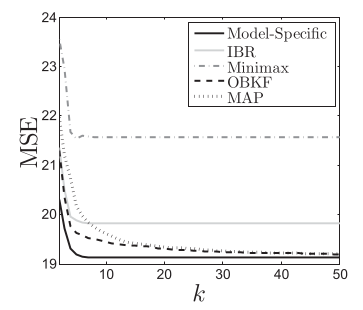
\includegraphics[width=7cm]{img/OBKF_r1.png}
    \caption{Performance analysis for specific $\theta_1 = 1$ and known $\theta_2$  \protect\linebreak OBKF achieves the lowest MSE (cited from \cite{Dehghannasiri2018})}
    \label{fig:r_1}
    \end{center}
\end{figure}
\end{frame}

\begin{frame}{Performance: Data Efficiency}
    \pnote{
    * figureはthetaがunknownであるときに高いMSEを達成するのに必要なstep数kを示している。
    }
\begin{figure}[H]
    \begin{center}
    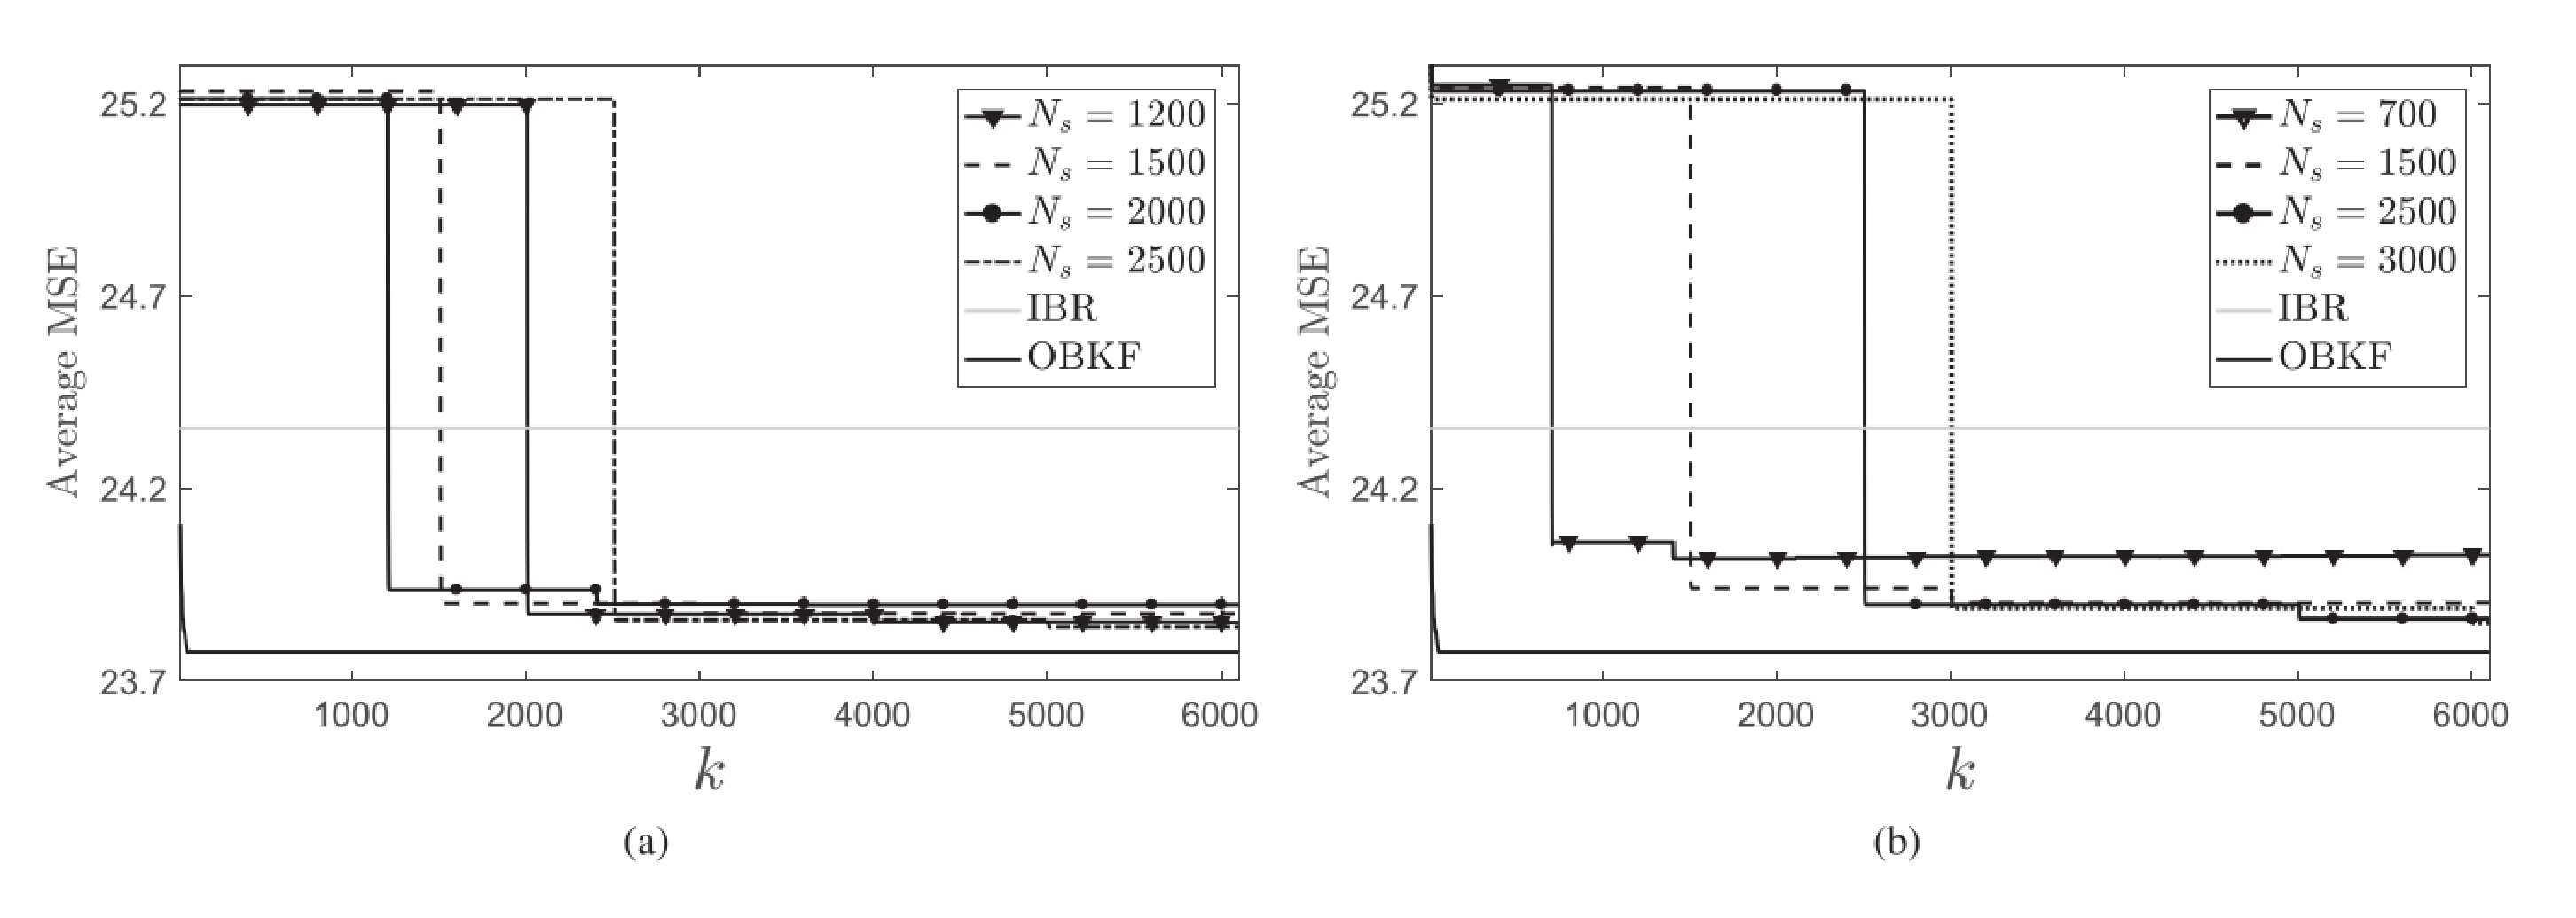
\includegraphics[width=9cm]{img/cmp_adaptive.eps}
    \caption{Unknown $\theta_1$ and comparison with an adaptive Kalman Filter (cited from \cite{Dehghannasiri2018})}
    \label{fig:cmp_adaptive}
    \end{center}
\end{figure}

\end{frame}


\subsection{Problems and Future Works}
\begin{frame}{Problems and Future Works}
\begin{itemize}
    \item If the prior distribution doesn't include the true value, the estimation won't converge
    \item Factor-graph and MCMC are computationally expensive. Finding an efficient approach is a future work.
\end{itemize}
\end{frame}
\section{Summery}
\begin{frame}
    \tableofcontents[currentsection]
\end{frame}

\begin{frame}{Summery}
\begin{itemize}
    \item OBKF converges to the optimal estimation as long as the prior distribution includes the true value
    \item OBKF requires much less data compared to Non-Bayesian methods
    \item The computational cost and deciding prior distribution are problems
\end{itemize}
\end{frame}

\begin{frame}[allowframebreaks]{References}
\nocite{*} 
\bibliographystyle{apalike} 
\bibliography{mybib} 

\end{frame}

\end{document} 